
\documentclass{article}
\usepackage[utf8]{inputenc}
\usepackage{graphicx}
\usepackage{textcomp}
\usepackage[margin=0.5in]{geometry}
\usepackage{array}
\usepackage{multirow}
\usepackage{hyperref}
\usepackage{xcolor}
\usepackage{booktabs}
\usepackage{amsmath}
\usepackage{amssymb}
\usepackage{float}
\usepackage{subcaption}
\usepackage{placeins}

\raggedbottom

\title{DSAA-6000Q Final Project Report\\Condition-Aware PEFT Selection for Instruction-Tuned LLMs}
\author{Team Members: Meijun Liu; Xiaoqian Jiao; Yiying Pan; Rui Liu \\ Date: May 12th, 2026}
\date{}

\begin{document}

\maketitle

\begin{abstract}
Parameter-efficient fine-tuning (PEFT) is a mainstream approach for adapting large language models under limited computation. However, existing research typically compares PEFT methods using average performance, failing to answer a critical practical question: which PEFT method should be chosen under different data budgets, model families, and task types? In this work, we conduct a controlled empirical study of four representative PEFT methods—LoRA, QLoRA, DoRA, and IA3—on two medium-sized instruction-tuned models. We evaluate reasoning, summarization, and question answering via GSM8K, DialogSum, and SQuAD v2, under three training budgets: 128, 512, and 2048 examples. The full experiment includes 144 runs across 2 models, 4 PEFT methods, 3 tasks, 3 budgets, and 2 random seeds. Beyond task performance, we measure GPU memory, training time, and trainable parameter ratios to analyze the efficiency–performance trade-off. Results show no single PEFT method universally dominates. Instead, the best method strongly depends on backbone, task, and budget. Specifically, QLoRA is the most memory-efficient, IA3 is the fastest to train, and the top-performing method shifts with budget on DialogSum and SQuAD v2. These findings support a condition-aware PEFT selection paradigm for real-world instruction-tuned LLM adaptation.
\end{abstract}

\section{Introduction}

Large language models (LLMs) have shown strong generalization ability across a wide range of downstream tasks, but adapting them through full-parameter fine-tuning is often expensive in terms of GPU memory, training time, and per-task storage. This challenge becomes even more salient in realistic deployment scenarios, where multiple downstream tasks may require repeated adaptation under limited computational budgets. For this reason, parameter-efficient fine-tuning (PEFT) has become the de facto standard to reduce cost while retaining performance. By freezing most pretrained parameters and updating only a small set of additional parameters or reparameterized modules, PEFT methods can significantly reduce training cost while preserving strong downstream performance \cite{hu2022lora,liu2022ia3,dettmers2023qlora}.

Although PEFT has become standard practice, method selection remains underexplored. In practical settings, researchers and practitioners often choose a PEFT method based on familiarity, implementation convenience, or isolated benchmark results. However, such choices may not transfer well across tasks, supervision budgets, or model families. A method that performs well in a low-data setting may not remain preferable when the training budget increases. Likewise, a method that is efficient on one model family may not show the same behavior on another. This suggests that PEFT selection should be treated as a conditional decision problem rather than a simple global ranking problem.

This issue is particularly important for instruction-tuned LLMs. Unlike traditional task-specific pretrained language models, instruction-tuned LLMs are designed to follow user instructions and support more general-purpose generation. As a result, adaptation settings are often more heterogeneous: tasks may involve reasoning, summarization, or evidence-based answering, and the trade-off between task quality and resource cost becomes more central. In this context, it is more meaningful to ask \emph{when} a PEFT method should be preferred, instead of asking \emph{which} method wins on average.

This project conducts a controlled empirical investigation into four representative PEFT methods, namely LoRA, QLoRA, DoRA, and IA3, for medium-sized instruction-tuned LLMs. Maintaining identical training pipelines, evaluation protocols, and logging procedures across all configurations, we conduct experiments covering two model families, three task types, and three data budgets, forming a 144-run experimental matrix. Instead of developing novel PEFT algorithms, this paper aims to provide empirical guidelines for practical PEFT selection by verifying whether optimal methods vary systematically under different constraints. We explicitly address four research questions:\begin{itemize}\item \textbf{RQ1:} Does the relative performance of different PEFT methods depend on data budget?\item \textbf{RQ2:} Does method preference change across model families?\item \textbf{RQ3:} How should task performance, memory usage, and training efficiency be jointly considered when selecting a PEFT method?\item \textbf{RQ4:} Does the 144-run matrix support a regime-dependent PEFT selection paradigm, instead of a universal global ranking?\end{itemize}

The main contributions of this work are summarized as follows. First, we redefine the PEFT selection task for instruction-tuned LLMs as a budget- and architecture-aware empirical comparison problem, rather than merely pursuing a universal average ranking. Second, we build a rigorous controlled experiment covering diverse PEFT techniques, model families, task types, data budgets, and random seeds within a unified training pipeline. Third, our analysis jointly evaluates task performance, memory consumption, training efficiency, and inherent trade-offs of each method, instead of focusing solely on benchmark accuracy. Finally, we deliver practical guidelines to assist researchers in selecting appropriate PEFT methods under varying model backbones, task scenarios, and resource constraints.



\section{Related Works}

Parameter-efficient fine-tuning has become a major research direction for adapting pretrained language models under limited computation and storage budgets. Early PEFT work includes prompt- and prefix-based approaches that optimize a small number of task-specific parameters while keeping the pretrained model fixed. Prefix-Tuning learns continuous task prefixes prepended to transformer layers \cite{li2021prefix}, while Prompt Tuning shows that soft prompts can become competitive when model scale is sufficiently large \cite{lester2021power}. These methods established the central PEFT idea that useful task adaptation does not necessarily require updating all model parameters.

Among weight-update methods, LoRA is the most influential baseline. It injects trainable low-rank matrices into selected linear projections and has become the standard reference point for PEFT comparisons \cite{hu2022lora}. Concretely, for a frozen weight matrix $W_0 \in \mathbb{R}^{d \times k}$, LoRA introduces a low-rank decomposition $\Delta W = BA$ where $B \in \mathbb{R}^{d \times r}$ and $A \in \mathbb{R}^{r \times k}$ with rank $r \ll \min(d,k)$. The forward pass becomes $h = W_0 x + \frac{\alpha}{r} BA x$, where $\alpha$ is a scaling hyperparameter. By keeping $r$ small (typically 8--64), LoRA reduces trainable parameters to under 1\% of the full model while maintaining competitive performance.

IA3 takes a different route by learning multiplicative rescaling vectors over activations instead of additive low-rank updates. Specifically, IA3 injects learned vectors $l_W$ into the key and value attention projections ($W_k$, $W_v$) and into the feed-forward block via element-wise multiplication: $h = (W x) \odot l_W$. This results in even fewer trainable parameters than LoRA---often below 0.01\% of the total---and its original study emphasizes both efficiency and few-shot competitiveness \cite{liu2022ia3}.

More recent work extends these paradigms in different directions. QLoRA combines 4-bit NormalFloat quantized model loading with LoRA-style updates to reduce memory cost without fully giving up downstream quality \cite{dettmers2023qlora}. The key innovation is the 4-bit NormalFloat (NF4) data type, which is information-theoretically optimal for normally distributed weights, combined with double quantization and paged optimizers to further reduce the memory footprint. DoRA revisits the low-rank update itself by decoupling weight magnitude and direction. Instead of directly learning $\Delta W$, DoRA decomposes the original weight into magnitude $m$ and directional component $V$, then applies LoRA only to the directional part: $W' = m \frac{V + \Delta V}{\|V + \Delta V\|_c}$. This aims to improve the expressiveness and robustness of LoRA-style adaptation \cite{liu2024dora}.

What is still missing in much of the literature is not evidence that PEFT works, but a clear answer to a more operational question: under a fixed model family, task type, and supervision budget, which method should be preferred? Existing papers usually establish the value of a single method or compare methods under limited settings. They are less often designed as controlled selection studies with multiple backbones, multiple task types, and explicit budget sweeps. This gap becomes more visible in instruction-tuned LLM settings, where task formats are heterogeneous and resource constraints matter in practice. Our work focuses on this empirical selection problem itself. Instead of proposing a new PEFT algorithm, we ask how method preference changes with budget, model family, and task type under a unified implementation environment. In this sense, our work is closer to a practical decision framework than a purely algorithmic contribution.

\section{Methodology}

 Overview of the full pipeline used in this study is shown in Figure~\ref{fig:workflow}. We treat the methodology as seven coordinated stages: (1) data collection and instruction-style pre-processing for the three target tasks; (2) selection of two medium-sized instruction-tuned backbones; (3) implementation of four PEFT families with their characteristic update structures; (4) a shared training configuration with method-specific knobs; (5) a $4 \times 2 \times 3 \times 3 \times 2 = 144$ training matrix plus six no-adaptation baselines, all logged with VRAM, wall-clock time, and trainable-parameter ratio; (6) task-performance and efficiency evaluation on a fixed 200-example evaluation slice per task; and (7) aggregation, ranking, and trade-off analysis. The subsections below describe each stage in detail.

\begin{figure}[H]
\centering
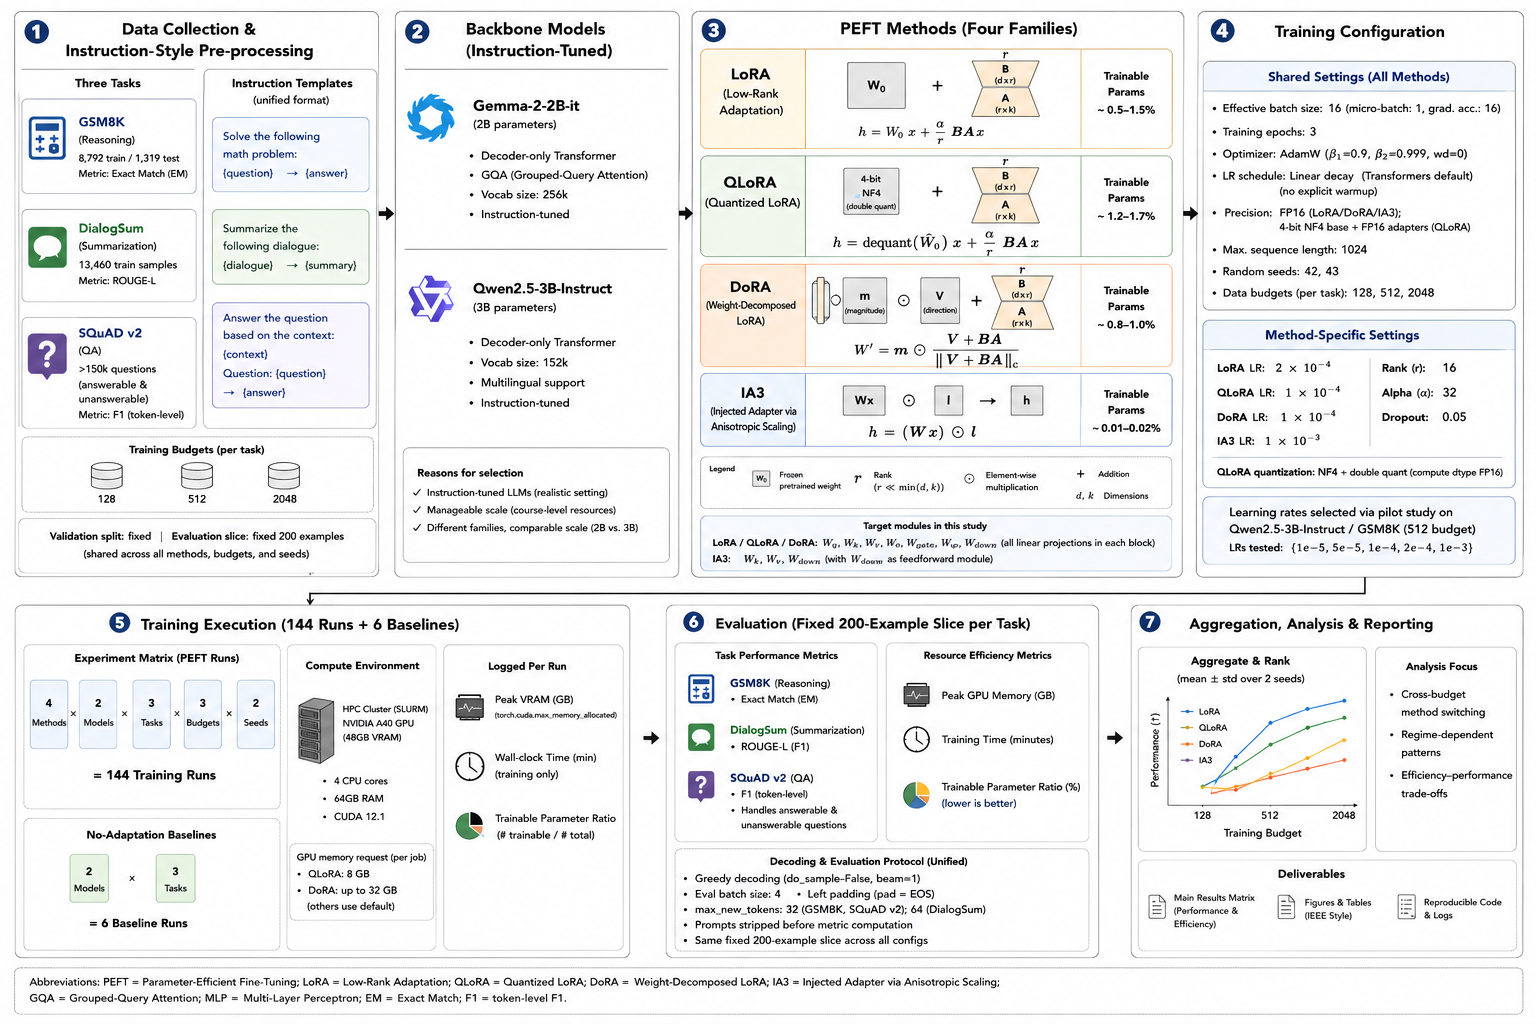
\includegraphics[width=\textwidth]{figures/Workflow.png}
\caption{End-to-end methodology pipeline. From left to right, top to bottom: task data and instruction templates, backbone selection, the four PEFT update equations and trainable-parameter ranges, the shared training configuration, the 144-run execution matrix with logged efficiency metrics, the evaluation metrics, and the downstream aggregation and analysis. The numerical hyperparameter values shown in the figure are illustrative; for the exact settings used in the experiments, refer to Table~\ref{tab:hyperparams}.}
\label{fig:workflow}
\end{figure}

\subsection{Data Collection and Pre-processing}

We evaluate PEFT methods on three tasks that reflect different types of instruction-tuned LLM usage: reasoning, summarization, and question answering.

\paragraph{Reasoning: GSM8K.} We use GSM8K as the reasoning task. GSM8K is a benchmark of grade-school mathematical word problems and is widely used for evaluating multi-step reasoning ability \cite{cobbe2021gsm8k}. The dataset contains 8,792 training and 1,319 test problems, each requiring 2--8 steps of arithmetic reasoning. We report Exact Match (EM) as the main metric.

\paragraph{Summarization: DialogSum.} We use DialogSum as the summarization task. DialogSum contains 13,460 dialogue-summary pairs drawn from real-life conversations and is suitable for evaluating instruction-conditioned summarization \cite{chen2021dialogsum}. The dialogues cover diverse domains including daily life, travel, and business meetings. We report ROUGE-L as the main metric.

\paragraph{Question Answering: SQuAD v2.} We use SQuAD v2 as the QA task. SQuAD v2 contains over 150,000 questions, including both answerable and unanswerable questions, which makes it appropriate for evaluating context-grounded answering behavior and the model's ability to identify when no answer exists \cite{rajpurkar2018squad2}. We report F1 as the primary metric, since exact-match evaluation is overly sensitive to generation format in decoder-only LLM evaluation.

For all three datasets, we convert the original inputs into a unified instruction-response format using task-specific prompt templates. For example, GSM8K instances are formatted as ``\texttt{Solve the following math problem: \{question\}}'' with the target answer as the response. DialogSum instances use the format ``\texttt{Summarize the following dialogue: \{dialogue\}}''. SQuAD v2 instances follow ``\texttt{Answer the question based on the context: \{context\} Question: \{question\}}''. We construct three training-budget subsets for each dataset: 128, 512, and 2048 training examples. Validation and evaluation splits are kept fixed across methods to ensure comparability. In the final main matrix, task metrics are reported on a fixed 200-example evaluation subset for each setting.

\subsection{Model Architecture}

We use two medium-sized instruction-tuned LLMs as backbone models:
\begin{itemize}
    \item \textbf{Gemma-2-2B-it} \cite{gemma2_2024}: A 2-billion parameter model from Google, trained with instruction tuning for general-purpose dialogue and task-following. It uses a decoder-only transformer architecture with grouped-query attention and a vocabulary size of 256k.
    \item \textbf{Qwen2.5-3B-Instruct} \cite{qwen25_2024}: A 3-billion parameter model from Alibaba Cloud, also instruction-tuned for diverse task performance. It features a 152k vocabulary with extended multilingual support.
\end{itemize}

These two models are chosen for three reasons. First, both are instruction-tuned LLMs, which aligns with the project goal of studying PEFT in realistic instruction-following settings. Second, their scale is manageable under course-level computational resources while still being large enough to exhibit meaningful scaling behaviors. Third, they belong to different model families and have comparable scale (2B vs.\ 3B), allowing us to examine whether PEFT method preference is architecture-sensitive rather than tied to a single backbone family.

\subsection{PEFT Methods}

We compare four PEFT methods that represent distinct design philosophies: additive low-rank decomposition (LoRA), quantized low-rank adaptation (QLoRA), magnitude--direction decomposition (DoRA), and multiplicative activation rescaling (IA3). Each method modifies the forward pass of selected transformer layers differently, resulting in varying trade-offs between expressiveness, parameter efficiency, and memory footprint. We present the formal definition of each method below.

\subsubsection{LoRA: Low-Rank Adaptation}

LoRA hypothesizes that the changes required to adapt a pretrained model to a downstream task reside in a low ``intrinsic rank'' subspace \cite{hu2022lora}. Given a frozen pretrained weight matrix $W_0 \in \mathbb{R}^{d \times k}$ in a linear layer, LoRA constrains the weight update by decomposing it into the product of two low-rank matrices:
\begin{equation}
\label{eq:lora_decomp}
\Delta W = BA, \quad B \in \mathbb{R}^{d \times r}, \quad A \in \mathbb{R}^{r \times k}
\end{equation}
where $r \ll \min(d, k)$ is the rank hyperparameter. Matrix $A$ is initialized with a random Gaussian distribution and $B$ is initialized to zero, so that $\Delta W = BA = 0$ at the start of training. The modified forward pass becomes:
\begin{equation}
\label{eq:lora_forward}
h = W_0 x + \frac{\alpha}{r} \Delta W \, x = W_0 x + \frac{\alpha}{r} BA \, x
\end{equation}
where $\alpha$ is a scaling factor that controls the magnitude of the low-rank update relative to the pretrained weights, and the division by $r$ ensures consistent scaling across different rank choices. During training, $W_0$ remains frozen and only $A$ and $B$ receive gradient updates. After training, the update can be merged into the original weight as $W = W_0 + \frac{\alpha}{r} BA$ for deployment, incurring no additional inference latency. The number of trainable parameters per adapted layer is $2dr$, which is typically less than 1\% of the original layer when $r$ is small. In our experiments we use $r = 16$ with $\alpha = 32$ and a LoRA dropout of $0.05$, and we attach LoRA adapters to all linear projections in every transformer block: the four attention projections ($W_q$, $W_k$, $W_v$, $W_o$) and the three MLP projections ($W_{\text{gate}}$, $W_{\text{up}}, W_{\text{down}}$). This broader target set, rather than the original LoRA paper's $\{W_q, W_v\}$-only configuration, follows recent practice for modern LLaMA-/Qwen-style backbones and yields the trainable-parameter ratios reported in Table~\ref{tab:trainable}.

\subsubsection{QLoRA: Quantized Low-Rank Adaptation}

QLoRA extends LoRA by combining 4-bit quantized model loading with full-precision low-rank adapters \cite{dettmers2023qlora}. The frozen backbone weights are stored in the 4-bit NormalFloat (NF4) data type, which is designed to be information-theoretically optimal for representing normally distributed weights. Given a pretrained weight tensor $W_0$, QLoRA first computes a normalization constant and maps each weight to one of $2^4 = 16$ quantile bins:
\begin{equation}
\label{eq:qlora_quant}
\hat{W}_0 = \text{quant}_{\text{NF4}}(W_0 / c), \quad c = \frac{\max(|W_0|)}{2^{b - 1}}
\end{equation}
where $b = 4$ is the number of bits and $c$ is the block-wise normalization constant. Double quantization is applied on top: the quantization constants $c$ themselves are further quantized to save additional memory. During the forward pass, the quantized weights are dequantized on-the-fly to compute in higher precision:
\begin{equation}
\label{eq:qlora_forward}
h = \text{dequant}(\hat{W}_0) \, x + \frac{\alpha}{r} BA \, x
\end{equation}
The LoRA adapters $B$ and $A$ remain in higher precision throughout training (FP16 in our implementation), and gradients flow through the adapter path while the quantized backbone provides memory savings. The original QLoRA paper additionally introduces paged optimizers; we keep the standard AdamW optimizer in our implementation and rely on quantization alone. QLoRA retains the same low-rank adapter structure as LoRA (Equation~\ref{eq:lora_decomp}); in our setting it reduces peak GPU memory relative to full-precision LoRA by a factor that depends on the backbone and matrix shapes (e.g., roughly $1.7\times$ on Gemma-2-2B-it and $2.8\times$ on Qwen2.5-3B-Instruct in our runs).

\subsubsection{DoRA: Weight-Decomposed Low-Rank Adaptation}

DoRA decomposes each pretrained weight matrix into its magnitude and directional components, then applies LoRA-style updates only to the directional part \cite{liu2024dora}. Given a frozen weight $W_0 \in \mathbb{R}^{d \times k}$, DoRA first computes the column-wise decomposition:
\begin{equation}
\label{eq:dora_decomp}
m = \|W_0\|_c, \quad V = \frac{W_0}{\|W_0\|_c}
\end{equation}
where $\|\cdot\|_c$ denotes the column-wise $\ell_2$ norm, producing a magnitude vector $m \in \mathbb{R}^k$ and a unit-norm directional matrix $V \in \mathbb{R}^{d \times k}$. A low-rank update $\Delta V = BA$ is then applied to the directional component, and the final adapted weight is reconstructed as:
\begin{equation}
\label{eq:dora_update}
W' = m \odot \frac{V + BA}{\|V + BA\|_c}
\end{equation}
where $\odot$ denotes column-wise multiplication (broadcasting $m$ across rows). Both the magnitude vector $m$ and the low-rank matrices $B$, $A$ are trainable. By separating magnitude from direction, DoRA allows the adapter to independently control the scaling of each output dimension (via $m$) and the representational direction of the update (via $\Delta V$). This decoupling is motivated by the observation that standard LoRA entangles magnitude and direction changes in a single $\Delta W$, which may limit its ability to mimic the learning patterns observed in full fine-tuning. The trainable parameter count is slightly higher than LoRA due to the additional magnitude vector.

\subsubsection{IA3: Injected Adapter via Anisotropic Scaling}

IA3 takes a fundamentally different approach from the additive low-rank methods above: instead of learning additive updates to weight matrices, it learns multiplicative rescaling vectors that are applied element-wise to intermediate activations \cite{liu2022ia3}. Given a weight projection $W$ in a transformer layer (e.g., attention key, value, or feed-forward projections), IA3 injects a learned vector $l_W$ of the same dimension as the output:
\begin{equation}
\label{eq:ia3_rescale}
h = (W x) \odot l_W
\end{equation}
where $\odot$ denotes element-wise multiplication. In the attention mechanism, IA3 applies separate learned vectors to the key and value projections:
\begin{equation}
\label{eq:ia3_attn}
k' = (W_k x) \odot l_k, \quad v' = (W_v x) \odot l_v
\end{equation}
In the feed-forward network, a single vector $l_{\text{FFN}}$ rescales the activations of the MLP down-projection ($W_{\text{down}}$, the second linear layer that maps the intermediate representation back to the model dimension). In our implementation $W_{\text{down}}$ is also flagged as the IA3 \emph{feedforward module}, so the rescaling is applied on the feed-forward side of the block rather than on the up-projection. The rescaling vectors $l_k$, $l_v$, and $l_{\text{FFN}}$ are initialized to all-ones vectors, so that the initial behavior is identical to the unmodified pretrained model. The total number of trainable parameters is $\sum_i d_i$, where $d_i$ is the hidden dimension of each rescaled layer. This results in significantly fewer trainable parameters than LoRA: typically 0.01--0.02\% of the total model, compared to LoRA's 0.5--1.5\%. The element-wise nature of the update makes IA3 extremely lightweight in both memory and computation, though its limited capacity may restrict performance on tasks that require more expressive adaptation.

\paragraph{Parameter efficiency comparison.}
Table~\ref{tab:trainable} summarizes the trainable parameter ratios for each method on both backbones. The differences span roughly two orders of magnitude, from IA3's sub-0.01\% to QLoRA's $\sim$1.7\%. This range directly affects VRAM consumption and training speed, as we discuss in Section~\ref{sec:efficiency}.

\begin{table}[H]
\centering
\small
\caption{Trainable parameter ratios for each PEFT method and backbone model.}
\label{tab:trainable}
\begin{tabular}{lcccc}
\toprule
Model & LoRA & QLoRA & DoRA & IA3 \\
\midrule
Gemma-2-2B-it & 0.788\% & 1.280\% & 0.815\% & 0.011\% \\
Qwen2.5-3B-Instruct & 0.961\% & 1.732\% & 0.993\% & 0.013\% \\
\bottomrule
\end{tabular}
\end{table}

\subsection{Training Configuration}

All methods are implemented using the Hugging Face Transformers library (v4.40) \cite{wolf2020transformers} with the PEFT extension (v0.11) \cite{peft2022} and PyTorch 2.3. We use a custom training loop built on the \texttt{Trainer} API, with unified scripts for data formatting, training, evaluation, and metric logging. Table~\ref{tab:hyperparams} summarizes the shared and method-specific hyperparameters.

\begin{table}[H]
\centering
\small
\caption{Training hyperparameters. Shared settings apply to all methods; method-specific settings are listed separately.}
\label{tab:hyperparams}
\begin{tabular}{@{}ll@{}}
\toprule
Hyperparameter & Value \\
\midrule
\multicolumn{2}{@{}l}{\textit{Shared settings}} \\
\midrule
Batch size (effective) & 16 \\
\quad Micro-batch size & 1 \\
\quad Gradient accumulation steps & 16 \\
Training epochs & 3 \\
Optimizer & AdamW ($\beta_1\!=\!0.9$, $\beta_2\!=\!0.999$, weight decay $0$) \\
Learning rate schedule & Linear decay (Transformers default; no explicit warmup) \\
Precision & FP16 (LoRA / DoRA / IA3); 4-bit NF4 base + FP16 adapters (QLoRA) \\
Max.\ sequence length & 1024 \\
Random seeds & 42, 43 \\
Data budgets (per task) & 128, 512, 2048 \\
\midrule
\multicolumn{2}{@{}l}{\textit{Method-specific settings}} \\
\midrule
LoRA learning rate & $2 \times 10^{-4}$ \\
QLoRA learning rate & $1 \times 10^{-4}$ \\
DoRA learning rate & $1 \times 10^{-4}$ \\
IA3 learning rate & $1 \times 10^{-3}$ \\
LoRA rank ($r$) & 16 \\
LoRA $\alpha$ & 32 \\
LoRA dropout & 0.05 \\
LoRA / QLoRA / DoRA target modules & $W_q, W_k, W_v, W_o, W_{\text{gate}}, W_{\text{up}}, W_{\text{down}}$ \\
QLoRA quantization & NF4 + double quantization (compute dtype FP16) \\
IA3 target modules & $W_k$, $W_v$, $W_{\text{down}}$ (with $W_{\text{down}}$ as feedforward module) \\
\bottomrule
\end{tabular}
\end{table}

The method-specific learning rates were determined through a pilot study on Qwen2.5-3B-Instruct with GSM8K under the 512-example budget, where we tested each method with learning rates in $\{1 \times 10^{-5}, 5 \times 10^{-5}, 1 \times 10^{-4}, 2 \times 10^{-4}, 1 \times 10^{-3}\}$. The selected rates follow a consistent pattern: IA3, which uses multiplicative rescaling with very few parameters, benefits from a larger learning rate ($1 \times 10^{-3}$), consistent with the original paper's recommendation. The additive low-rank methods (LoRA, QLoRA, DoRA) use smaller rates ($1\text{--}2 \times 10^{-4}$) to ensure stable convergence, with LoRA receiving the highest among them due to its simpler update mechanism.

Our main experiment matrix is:
\[
4 \text{ methods} \times 2 \text{ models} \times 3 \text{ tasks} \times 3 \text{ budgets} \times 2 \text{ seeds} = 144 \text{ runs}.
\]
Each run trains a single PEFT adapter on one model for one task-budget-seed combination. Beyond the 144 PEFT runs, we additionally evaluate 6 no-adaptation baselines (2 models $\times$ 3 tasks) to establish reference scores without fine-tuning.

\subsection{Computational Resources}

All experiments are conducted on a university high-performance computing (HPC) cluster equipped with NVIDIA A40 GPUs (48 GB VRAM, Ampere architecture, CUDA 12.1). Each training run is allocated a single GPU with 4 CPU cores and 64 GB of system RAM. The HPC cluster uses a SLURM job scheduler, and each job requests resources based on the PEFT method: QLoRA runs use 8 GB GPU memory, while DoRA runs request up to 32 GB to accommodate the larger memory footprint.

To enable a rigorous efficiency analysis, we log three resource metrics for every run. First, peak VRAM usage is recorded via \texttt{torch.cuda.max\_memory\_allocated()}, which reports the maximum GPU memory consumed during training, including model weights, gradients, optimizer states, and intermediate activations. Second, training wall-clock time is measured from the start of the first training epoch to the completion of the last, excluding data downloading and model loading time. Third, the trainable parameter ratio is computed as the number of updated parameters divided by the total model parameters, providing a normalized measure of method complexity.

These three metrics capture the key dimensions of the efficiency--performance trade-off. Peak VRAM determines whether a method can be deployed on a given GPU, wall-clock time reflects the practical cost of repeated adaptation, and the trainable parameter ratio indicates the storage overhead of maintaining task-specific adapters.

\subsection{Evaluation Metrics}

We evaluate each PEFT configuration from two complementary perspectives: task performance and resource efficiency. All task metrics are computed on a fixed 200-example evaluation subset that is held out from training and shared across all methods to ensure direct comparability.

\paragraph{Task performance metrics.}
For GSM8K, we report Exact Match (EM), which requires the generated answer to exactly match the ground-truth numeric answer after normalization (stripping whitespace, commas, and currency symbols). For DialogSum, we report ROUGE-L \cite{lin2004rouge}, the F1 score based on the longest common subsequence between the generated summary and the reference summary, which captures both precision and recall of salient content. For SQuAD v2, we report token-level F1 following the official evaluation script, which accounts for both answerable and unanswerable questions by assigning zero credit when the model fails to predict ``no answer'' for unanswerable instances.

\paragraph{Resource efficiency metrics.}
We report three resource metrics. Peak GPU memory usage (GB) is the maximum VRAM allocated during training, including model parameters, gradients, and optimizer states. Training wall-clock time (minutes) measures the total time from the start of the first epoch to the end of the last, providing a practical measure of computational cost. Trainable parameter ratio is the fraction of total model parameters that receive gradient updates during training, reflecting the storage overhead of each adapter method.

\paragraph{Decoding and evaluation protocol.}
All evaluation is performed with the same generation setup to keep comparisons fair. We use greedy decoding (\texttt{do\_sample=False}, beam size 1), an evaluation batch size of 4, and left padding with the EOS token treated as the pad token. The generation budget is task-specific: \texttt{max\_new\_tokens}=32 for GSM8K and SQuAD v2, and \texttt{max\_new\_tokens}=64 for DialogSum, reflecting the typical length of the target answer or summary. For each task we evaluate on a fixed 200-example slice taken from the GSM8K \texttt{test} split, the DialogSum \texttt{test} split, and the SQuAD v2 \texttt{validation} split. The same slice is reused across all methods, budgets, and seeds, so any difference between configurations is attributable to the model and adapter rather than to evaluation sampling. After generation, the echoed prompt prefix is stripped from the decoded output before metric computation, and SQuAD v2 answers are normalized following the official script (lowercasing, article and punctuation removal, whitespace collapsing).

\paragraph{Aggregation and reproducibility.}
Each configuration (model, method, task, budget) is run with two random seeds (42 and 43). We report the mean and standard deviation across seeds as the primary performance estimate. Because our evaluation set is limited to 200 examples per task and the generation budget is short, we focus on relative method comparisons within the same model--task setting rather than on absolute score benchmarks. The main analysis examines cross-budget method switching and regime-dependent patterns rather than step-level training dynamics.

\section{Results}

\subsection{Main Performance Results}

Tables~\ref{tab:gsm8k}, \ref{tab:dialogsum}, and \ref{tab:squad} summarize the mean performance across two random seeds. Overall, the results show that PEFT method preference is not uniform across all conditions. Instead, the relative ranking of methods changes with data budget, task type, and, in several cases, model family. This already suggests that average ranking alone is insufficient for practical method selection.

Figure~\ref{fig:main_bar} provides a visual overview of all task results across both models. The grouped bar chart format allows direct comparison of methods within each budget level, while the error bars convey the variance across seeds.

\begin{figure}[H]
\centering

\includegraphics[width=\textwidth]{figures/fig1_main_results_bar.png}
\caption{Main results overview: mean performance of four PEFT methods across three data budgets (128, 512, 2048) for each task and model combination. Error bars indicate standard deviation over two random seeds. Each row corresponds to a model, each column to a task.}
\label{fig:main_bar}
\end{figure}

Several high-level patterns are visible from Figure~\ref{fig:main_bar}. The gap between Gemma and Qwen is largest on SQuAD v2, where Gemma achieves F1 scores roughly 4--5$\times$ higher than Qwen. On DialogSum, the relative differences across methods are larger than on the other tasks. On GSM8K, absolute performance is low for both models (EM $<$ 8\%). Importantly, no single method consistently outperforms the others; the best method changes with both budget and model, providing the first evidence for regime-dependent PEFT selection.

We now report the detailed numerical results. Tables~\ref{tab:gsm8k}, \ref{tab:dialogsum}, and~\ref{tab:squad} present the mean $\pm$ standard deviation for every configuration, with the best method per model per budget shown in \textbf{bold}. All values are multiplied by 100 and presented as percentages.

\begin{table}[H]
\centering
\small
\caption{GSM8K exact match accuracy (\%). Reported as mean $\pm$ std over two random seeds. The best method for each model at each budget is \textbf{bolded}.}
\label{tab:gsm8k}
\begin{tabular}{@{}llccc@{}}
\toprule
Model & Method & \multicolumn{3}{c@{}}{Training Examples} \\
\cmidrule(l){3-5}
 & & 128 & 512 & 2\,048 \\
\midrule
\multirow{4}{*}{Gemma-2-2B-it}
 & LoRA  & $3.75 \pm 0.35$ & $1.50 \pm 0.00$ & $0.75 \pm 0.35$ \\
 & QLoRA & $6.25 \pm 1.06$ & $1.50 \pm 0.00$ & $1.75 \pm 1.06$ \\
 & DoRA  & $\mathbf{7.50} \pm 1.41$ & $2.00 \pm 0.71$ & $1.50 \pm 0.00$ \\
 & IA3   & $3.50 \pm 0.00$ & $\mathbf{5.75} \pm 0.35$ & $\mathbf{4.25} \pm 0.35$ \\
\midrule
\multirow{4}{*}{Qwen2.5-3B-Instruct}
 & LoRA  & $1.75 \pm 0.35$ & $1.50 \pm 0.71$ & $1.50 \pm 1.41$ \\
 & QLoRA & $\mathbf{3.00} \pm 1.41$ & $\mathbf{3.50} \pm 1.41$ & $\mathbf{2.75} \pm 1.06$ \\
 & DoRA  & $2.25 \pm 0.35$ & $1.75 \pm 0.35$ & $2.00 \pm 0.00$ \\
 & IA3   & $1.50 \pm 0.71$ & $2.00 \pm 0.71$ & $2.50 \pm 0.71$ \\
\bottomrule
\end{tabular}
\end{table}

\begin{table}[H]
\centering
\small
\caption{DialogSum ROUGE-L score (\%). Reported as mean $\pm$ std over two random seeds. The best method for each model at each budget is \textbf{bolded}.}
\label{tab:dialogsum}
\begin{tabular}{@{}llccc@{}}
\toprule
Model & Method & \multicolumn{3}{c@{}}{Training Examples} \\
\cmidrule(l){3-5}
 & & 128 & 512 & 2\,048 \\
\midrule
\multirow{4}{*}{Gemma-2-2B-it}
 & LoRA  & $26.62 \pm 0.21$ & $\mathbf{31.14} \pm 0.18$ & $30.69 \pm 0.66$ \\
 & QLoRA & $27.17 \pm 0.21$ & $30.78 \pm 0.39$ & $\mathbf{32.43} \pm 1.04$ \\
 & DoRA  & $\mathbf{27.30} \pm 0.74$ & $29.61 \pm 0.26$ & $31.69 \pm 1.92$ \\
 & IA3   & $25.33 \pm 0.18$ & $29.22 \pm 0.04$ & $27.86 \pm 0.14$ \\
\midrule
\multirow{4}{*}{Qwen2.5-3B-Instruct}
 & LoRA  & $\mathbf{21.31} \pm 0.01$ & $21.07 \pm 0.39$ & $21.55 \pm 0.11$ \\
 & QLoRA & $19.17 \pm 0.02$ & $\mathbf{22.33} \pm 0.11$ & $20.71 \pm 0.27$ \\
 & DoRA  & $19.43 \pm 0.15$ & $21.66 \pm 0.37$ & $\mathbf{22.97} \pm 0.17$ \\
 & IA3   & $18.40 \pm 0.12$ & $19.12 \pm 0.05$ & $19.77 \pm 0.14$ \\
\bottomrule
\end{tabular}
\end{table}

On GSM8K, all methods achieve relatively low absolute EM (below 8\%), and the differences across methods are modest. Two factors jointly explain this floor effect. First, GSM8K requires multi-step arithmetic reasoning, and learning such skills from only 128--2048 instruction-formatted examples is inherently difficult. Second, our evaluation uses a short generation budget (\texttt{max\_new\_tokens}=32) and a lightweight ``last-number'' extraction rule, so chains of reasoning that are correct but unfinished, or finished but trailing extra digits, are penalized; the reported EM therefore underestimates the underlying reasoning capability and should be interpreted as a comparative signal across methods rather than an absolute capability score. With this caveat in mind, the relative pattern is still informative: on Qwen, QLoRA is consistently the best option across all three budgets; on Gemma, the best method changes from DoRA at budget 128 to IA3 at budgets 512 and 2048, indicating that increasing the training budget does not produce a simple monotonic improvement in this reasoning setting.

On DialogSum, the relative differences are clearer and the preferred method changes with budget on both backbones. On Gemma, the winner shifts from DoRA at 128 to LoRA at 512 and QLoRA at 2048. On Qwen, the winner shifts from LoRA at 128 to QLoRA at 512 and DoRA at 2048. This clean switching pattern strongly supports the central premise of the project: PEFT selection should be understood as a conditional choice problem. The standard deviations are generally small ($<$ 1.0 on the percentage scale), confirming that the method-switching patterns are robust to seed variation.

\begin{table}[H]
\centering
\small
\caption{SQuAD v2 F1 score (\%). Reported as mean $\pm$ std over two random seeds. The best method for each model at each budget is \textbf{bolded}.}
\label{tab:squad}
\begin{tabular}{@{}llccc@{}}
\toprule
Model & Method & \multicolumn{3}{c@{}}{Training Examples} \\
\cmidrule(l){3-5}
 & & 128 & 512 & 2\,048 \\
\midrule
\multirow{4}{*}{Gemma-2-2B-it}
 & LoRA  & $45.29 \pm 3.08$ & $\mathbf{59.04} \pm 2.86$ & $53.97 \pm 2.04$ \\
 & QLoRA & $49.29 \pm 1.50$ & $49.97 \pm 1.02$ & $48.97 \pm 2.49$ \\
 & DoRA  & $46.29 \pm 0.48$ & $55.40 \pm 2.99$ & $\mathbf{55.02} \pm 1.77$ \\
 & IA3   & $\mathbf{54.93} \pm 0.35$ & $54.84 \pm 0.00$ & $52.47 \pm 0.12$ \\
\midrule
\multirow{4}{*}{Qwen2.5-3B-Instruct}
 & LoRA  & $\mathbf{12.62} \pm 0.88$ & $\mathbf{10.84} \pm 0.13$ & $8.93 \pm 0.20$ \\
 & QLoRA & $9.47 \pm 0.03$ & $7.22 \pm 1.67$ & $7.29 \pm 1.10$ \\
 & DoRA  & $9.71 \pm 0.13$ & $9.18 \pm 1.36$ & $\mathbf{9.20} \pm 0.31$ \\
 & IA3   & $9.18 \pm 0.10$ & $8.94 \pm 0.01$ & $8.53 \pm 0.08$ \\
\bottomrule
\end{tabular}
\end{table}

On SQuAD v2, the most striking effect is model family rather than PEFT method. Gemma is substantially stronger than Qwen across all budgets (F1 range 0.45--0.59 vs.\ 0.07--0.13), while the within-model best method still changes with budget. This indicates that backbone family can have a larger impact than method choice on certain tasks, even though regime-dependent method preference still exists inside each backbone.

\subsubsection{Performance Scaling with Data Budget}

To better understand how each method responds to changes in data availability, Figure~\ref{fig:scaling} plots task performance as a function of data budget for all model-method combinations. The line chart format highlights scaling trends: upward slopes indicate that a method benefits from more training data, while flat or downward slopes suggest diminishing returns or even degradation.

\begin{figure}[H]
\centering

\includegraphics[width=\textwidth]{figures/fig2_performance_vs_budget.png}
\caption{Performance scaling with data budget. Each panel corresponds to a task. Solid lines represent Gemma, dashed lines represent Qwen. Each color/marker combination indicates a PEFT method. The x-axis shows the training budget (128, 512, 2048) and the y-axis shows the task-specific metric.}
\label{fig:scaling}
\end{figure}

Several patterns emerge from Figure~\ref{fig:scaling}. On SQuAD-v2 (Gemma), LoRA and DoRA exhibit strong positive scaling, with LoRA achieving a notable peak at budget 512 (F1 = 59.04\%) before declining slightly at 2048. This non-monotonic behavior may indicate mild overfitting with the higher-capacity methods at larger budgets. IA3, by contrast, shows relatively flat scaling across budgets, consistent with its limited capacity due to extremely few trainable parameters. On DialogSum, most methods show upward trends, with DoRA and QLoRA displaying the most consistent improvement from budget 128 to 2048 on both models. For Qwen on GSM8K, all methods remain near zero across all budgets, confirming the difficulty of learning mathematical reasoning under these constraints.

\subsubsection{Score Distribution Heatmap}

Figure~\ref{fig:heatmap} presents the same results in heatmap form, providing a compact visual summary where darker cells indicate higher scores. This format makes it easy to identify the strongest configurations at a glance.

\begin{figure}[H]
\centering

\includegraphics[width=0.85\textwidth]{figures/fig9_score_heatmap.png}
\caption{Performance score heatmap showing mean task metric for each method-budget combination. Each panel corresponds to a model-task pair. Darker cells indicate higher performance.}
\label{fig:heatmap}
\end{figure}

The heatmap reveals a clear ``hot spot'' at Gemma + SQuAD v2 under LoRA with budget 512, representing the single best configuration in the entire study. Conversely, the GSM8K panels appear uniformly light for both models, reflecting the overall difficulty of this task. The color gradient along the budget axis varies by method and task, visually confirming that some methods benefit more from additional data than others.

\subsection{Best Method by Budget}

Table~\ref{tab:best} summarizes the best-performing method for each task, model, and budget. The pattern is highly structured. For DialogSum, the winning method changes as the training budget increases on both backbones. For SQuAD v2, Gemma prefers IA3 at 128, LoRA at 512, and DoRA at 2048, whereas Qwen prefers LoRA at 128 and 512, but DoRA at 2048. For GSM8K, Gemma favors DoRA only at the smallest budget and IA3 at higher budgets, while Qwen consistently favors QLoRA. These results reinforce the view that PEFT choice should not be based on a single global ranking.

\begin{table}[H]
\centering
\small
\caption{Best-performing method under each task, model, and budget. Scores are averaged over two seeds.}
\label{tab:best}
\begin{tabular}{llccc}
\toprule
Task & Model & 128 & 512 & 2048 \\
\midrule
GSM8K & Gemma-2-2B-it & DoRA (0.0750) & IA3 (0.0575) & IA3 (0.0425) \\
GSM8K & Qwen2.5-3B-Instruct & QLoRA (0.0300) & QLoRA (0.0350) & QLoRA (0.0275) \\
\midrule
SQuAD v2 & Gemma-2-2B-it & IA3 (0.5493) & LoRA (0.5904) & DoRA (0.5502) \\
SQuAD v2 & Qwen2.5-3B-Instruct & LoRA (0.1262) & LoRA (0.1084) & DoRA (0.0920) \\
\midrule
DialogSum & Gemma-2-2B-it & DoRA (0.2730) & LoRA (0.3114) & QLoRA (0.3243) \\
DialogSum & Qwen2.5-3B-Instruct & LoRA (0.2131) & QLoRA (0.2233) & DoRA (0.2297) \\
\bottomrule
\end{tabular}
\end{table}

Figure~\ref{fig:best_method} visualizes these results as a color-coded grid, making the method-switching pattern immediately visible. The color of each cell indicates which method won, and the numerical score is overlaid for reference.

\begin{figure}[H]
\centering

\includegraphics[width=0.85\textwidth]{figures/fig5_best_method_heatmap.png}
\caption{Best PEFT method for each task, model, and budget combination. Each cell shows the winning method name (top) and its score (bottom). Cell color indicates the method identity. The systematic change in winning method across budget levels illustrates the regime-dependent nature of PEFT selection.}
\label{fig:best_method}
\end{figure}

A particularly notable pattern is the ``switching point'' on Gemma + SQuAD v2: IA3 wins at the smallest budget (where its parameter efficiency is most advantageous), LoRA dominates at the intermediate budget, and DoRA takes over at the largest budget (where its higher expressiveness can be fully utilized). This three-way switching behavior directly addresses the TA's expectation that the study would identify such budget-dependent transitions.

\subsection{Cross-Architecture Comparison}

Method preference is not architecture-invariant. The clearest example is SQuAD v2: Gemma achieves F1 scores roughly in the range of 0.45--0.59, whereas Qwen remains in the much lower range of about 0.07--0.13. This indicates that backbone family can have a larger effect than PEFT method choice on certain tasks. Even when the best method changes with budget inside each backbone, the absolute performance gap between model families remains substantial.

To make the backbone effect more explicit, Table~\ref{tab:backbone_avg} reports the average task performance across all four PEFT methods for each model and budget. Gemma consistently outperforms Qwen on DialogSum and SQuAD v2 across all budgets, while GSM8K shows a smaller and less stable backbone gap. This confirms that model family is not just a secondary factor, but a major determinant of downstream adaptation quality in our setup. 

\begin{table}[H]
\centering
\small
\caption{Average task performance across all PEFT methods for each backbone and budget.}
\label{tab:backbone_avg}
\begin{tabular}{llccc}
\toprule
Task & Model & 128 & 512 & 2048 \\
\midrule
\multirow{2}{*}{GSM8K (EM)} & Gemma-2-2B-it & 0.0525 & 0.0269 & 0.0206 \\
 & Qwen2.5-3B-Instruct & 0.0213 & 0.0219 & 0.0219 \\
\midrule
\multirow{2}{*}{DialogSum (ROUGE-L)} & Gemma-2-2B-it & 0.2661 & 0.3019 & 0.3067 \\
 & Qwen2.5-3B-Instruct & 0.1958 & 0.2105 & 0.2125 \\
\midrule
\multirow{2}{*}{SQuAD v2 (F1)} & Gemma-2-2B-it & 0.4895 & 0.5481 & 0.5261 \\
 & Qwen2.5-3B-Instruct & 0.1024 & 0.0905 & 0.0849 \\
\bottomrule
\end{tabular}
\end{table}

Interestingly, despite Qwen2.5-3B having 1.5$\times$ more parameters than Gemma-2-2B, it underperforms on all three tasks. We do not claim a single mechanistic explanation for this gap; rather, several factors plausibly contribute, all of which would require dedicated ablations to disentangle. Candidate factors include: (1) sensitivity to the specific instruction template we used, which was tuned by inspection rather than by per-model prompt search; (2) differences in default generation behavior (e.g., chat-style formatting, repetition, or stop-token usage) that interact with our greedy short-generation evaluation; (3) per-method learning rates that were selected on a single Qwen + GSM8K + 512 cell and then transferred to all settings, which may favor one backbone over the other; and (4) architectural and training-recipe differences between the two model families that we cannot directly observe. Regardless of cause, the primary goal of this study is to compare PEFT methods \emph{within} each backbone, and the regime-dependent patterns hold consistently within both model families.

\subsection{Comparison with the Base Model}
\label{sec:base_comparison}

To contextualize the PEFT comparison, we additionally evaluate the original instruction-tuned backbone models without any adapter-based fine-tuning. This baseline is evaluated only at inference time and is therefore not associated with any training budget. As shown in Table~\ref{tab:base_vs_best}, PEFT consistently improves performance over the base model, but the magnitude of improvement is highly task-dependent.

\begin{table}[H]
\centering
\small
\caption{Comparison between base models and the best PEFT result for each model-task pair.}
\label{tab:base_vs_best}
\begin{tabular}{llccc}
\toprule
Model & Task & Base Score & Best PEFT & Gain \\
\midrule
Gemma-2-2B-it & DialogSum (ROUGE-L) & 0.2506 & 0.3243 (QLoRA) & +0.0737 \\
Gemma-2-2B-it & GSM8K (EM) & 0.0100 & 0.0750 (DoRA) & +0.0650 \\
Gemma-2-2B-it & SQuAD v2 (F1) & 0.5418 & 0.5904 (LoRA) & +0.0486 \\
Qwen2.5-3B-Instruct & DialogSum (ROUGE-L) & 0.1875 & 0.2297 (DoRA) & +0.0421 \\
Qwen2.5-3B-Instruct & GSM8K (EM) & 0.0150 & 0.0350 (QLoRA) & +0.0200 \\
Qwen2.5-3B-Instruct & SQuAD v2 (F1) & 0.1099 & 0.1262 (LoRA) & +0.0163 \\
\bottomrule
\end{tabular}
\end{table}

The magnitude of PEFT improvement varies substantially across tasks and models. On DialogSum, the gains are largest in both absolute and relative terms: Gemma improves by $+0.0737$ ROUGE-L (a $29.4\%$ relative gain over the base score of $0.2506$), and Qwen improves by $+0.0421$ ($22.5\%$ relative). On GSM8K, although the absolute gains appear modest, the relative improvement is striking---Gemma's EM jumps from $0.0100$ to $0.0750$, a $7.5\times$ increase. This suggests that even a small amount of task-specific adaptation can activate latent reasoning capabilities in instruction-tuned models that remain dormant under zero-shot inference. In contrast, the gains on SQuAD v2 are much smaller. Gemma is already strong before adaptation (base F1 $= 0.5418$), and the best PEFT result raises it only to $0.5904$ ($+9.0\%$ relative). Qwen shows even smaller gains on SQuAD v2, improving from $0.1099$ to $0.1262$ ($+14.8\%$ relative).

Two observations follow from this contrast. First, \textbf{the ceiling effect}: when the backbone already performs well on a task (as Gemma does on SQuAD v2), PEFT has limited room to improve, and the cost--benefit ratio of fine-tuning decreases. Second, \textbf{the backbone bottleneck}: when the backbone is weak on a task (as Qwen is on SQuAD v2, with F1 $<$ 0.13), PEFT alone cannot compensate---the bottleneck lies in the model's fundamental capability rather than in the absence of task-specific parameters. In such cases, investing in a stronger backbone model or in better pretraining data may yield higher returns than tuning the PEFT method. Together, these two effects argue that \emph{fine-tuning is not uniformly worth its cost}: before committing GPU hours and storage to an adapter sweep, it is worth checking whether the no-adaptation baseline is already near the achievable ceiling, or so far below it that PEFT will not close the gap. An additional pattern concerns which PEFT method delivers the best improvement. For Gemma, the optimal method differs by task: DoRA on GSM8K, QLoRA on DialogSum, and LoRA on SQuAD v2. This further reinforces the central finding that method preference is regime-dependent, extending even to the question of ``whether to fine-tune at all''---the answer depends on the task--backbone combination.

Figure~\ref{fig:base_vs_peft} visualizes the absolute scores of all PEFT methods alongside the base model baseline (gray dotted line), making it easy to see which configurations exceed the no-adaptation baseline and by how much.


\begin{figure}[H]
\centering
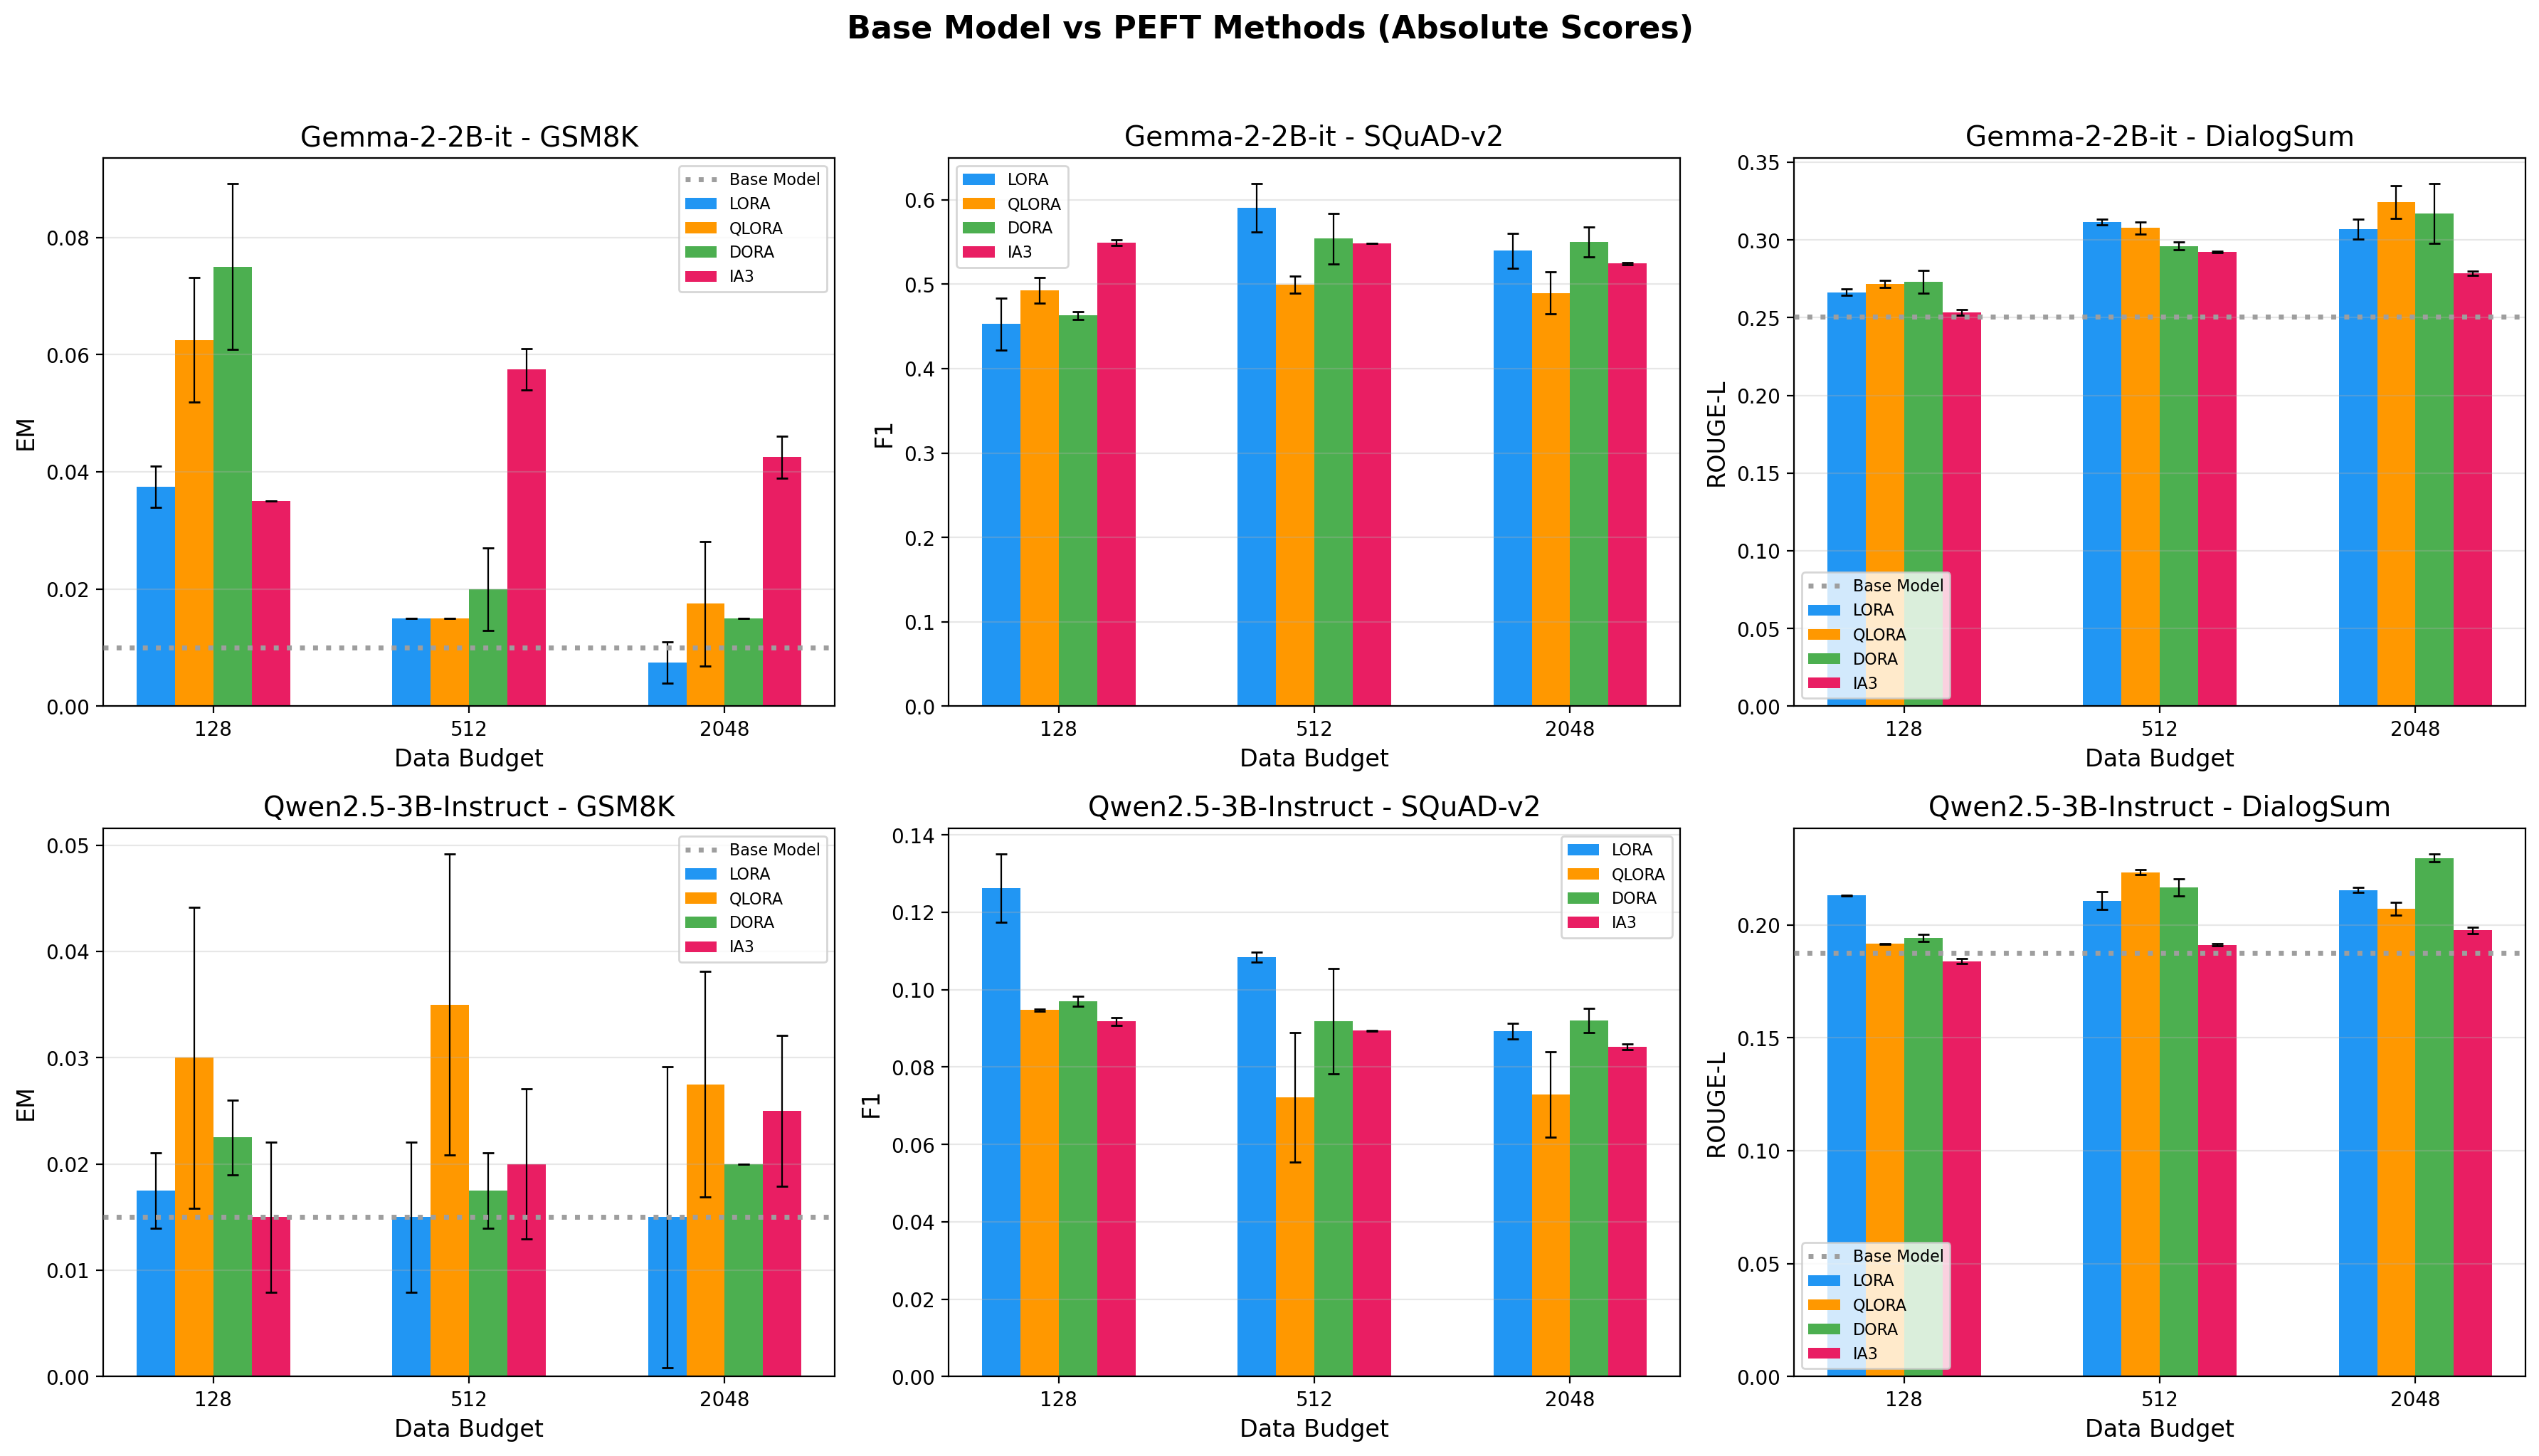
\includegraphics[width=\textwidth]{figures/fig12_base_vs_peft_absolute.png}
\caption{Base model vs PEFT methods (absolute scores). The gray dotted line in each panel indicates the base model score without any fine-tuning. All PEFT methods and budgets are shown for comparison. Panels where the base line sits near the PEFT bars (e.g., Qwen + GSM8K) indicate tasks where adaptation provides marginal gains.}
\label{fig:base_vs_peft}
\end{figure}

Figure~\ref{fig:delta_peft} further decomposes this comparison into the delta improvement over the base model. While Figure~\ref{fig:base_vs_peft} shows absolute scores, the delta view isolates the \emph{marginal benefit} of fine-tuning, making it easier to identify settings where PEFT investment is justified. The largest improvements appear on Gemma + DialogSum, where QLoRA at budget 2048 achieves a delta of $+0.0737$ in ROUGE-L. On Qwen + GSM8K and Qwen + SQuAD v2, the deltas are near zero, confirming that the backbone itself---rather than the PEFT method---is the performance bottleneck in these settings.

\begin{figure}[H]
\centering
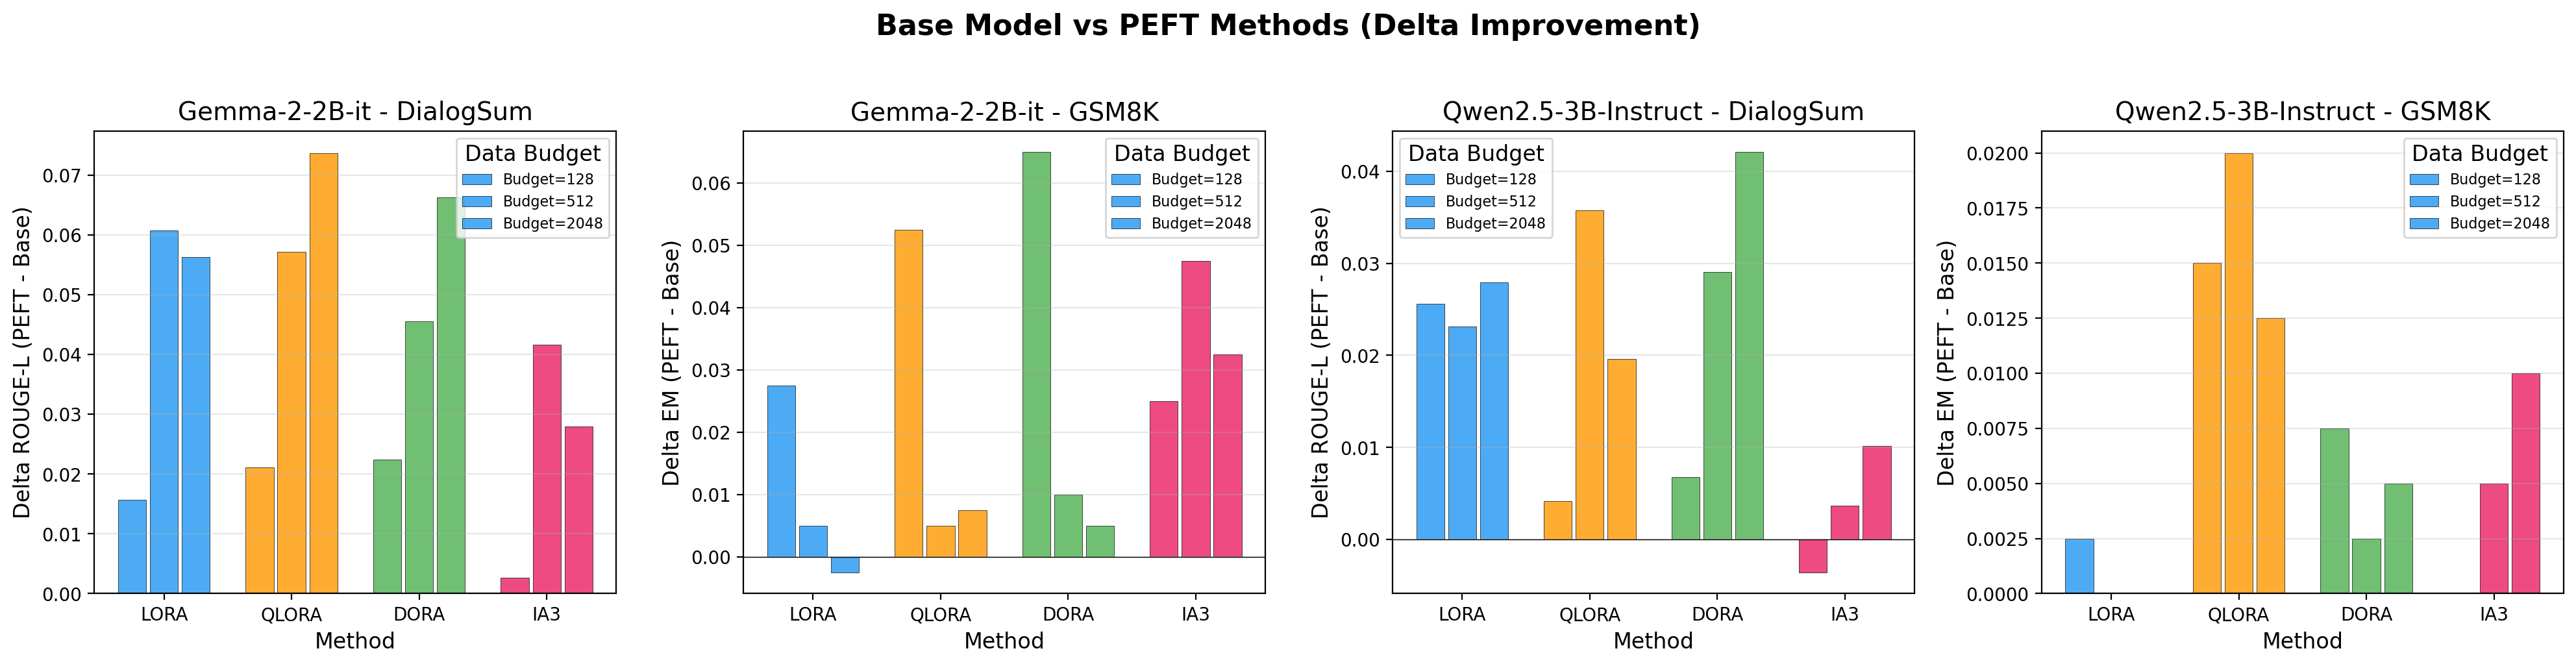
\includegraphics[width=1.0\textwidth]{figures/fig11_base_vs_peft_delta.png}
\caption{Delta improvement of PEFT methods over the base model. Only configurations with meaningful gains ($\Delta > 0.005$) are shown. Positive bars indicate configurations where fine-tuning improves over the raw instruction-tuned model.}
\label{fig:delta_peft}
\end{figure}

These results indicate that PEFT is not uniformly beneficial across all settings: in some regimes it provides substantial gains (especially on summarization and reasoning), while in others the backbone model itself is already the main determinant of final performance. This reinforces the importance of evaluating PEFT methods relative to a simple no-adaptation baseline before committing computational resources to fine-tuning.

\subsection{Efficiency--Performance Trade-off}
\label{sec:efficiency}

Beyond task performance, resource efficiency is a critical dimension for practical PEFT selection. Table~\ref{tab:efficiency} summarizes the average efficiency statistics across all tasks and budgets.

\begin{table}[H]
\centering
\small
\caption{Average efficiency statistics across all tasks, budgets, and seeds.}
\label{tab:efficiency}
\begin{tabular}{llccc}
\toprule
Model & Method & Peak VRAM (GB) & Train Time (min) & Trainable Ratio \\
\midrule
\multirow{4}{*}{Gemma-2-2B-it} & LoRA & 13.15 & 10.26 & 0.007881 \\
 & QLoRA & 7.65 & 22.24 & 0.012795 \\
 & DoRA & 19.65 & 19.57 & 0.008146 \\
 & IA3 & 12.11 & 8.00 & 0.000112 \\
\midrule
\multirow{4}{*}{Qwen2.5-3B-Instruct} & LoRA & 14.06 & 11.35 & 0.009607 \\
 & QLoRA & 5.00 & 23.64 & 0.017317 \\
 & DoRA & 23.17 & 23.61 & 0.009935 \\
 & IA3 & 12.71 & 7.09 & 0.000134 \\
\bottomrule
\end{tabular}
\end{table}

\subsubsection{Peak VRAM Usage}

\begin{figure}[H]
\centering

\includegraphics[width=0.85\textwidth]{figures/fig3_vram_usage.png}
\caption{Peak VRAM usage by PEFT method and model. Each panel shows the GPU memory consumption for one backbone model across all four methods and three data budgets. Error bars indicate standard deviation over seeds. Note that VRAM is determined by the method and model configuration, not by the training budget.}
\label{fig:vram}
\end{figure}

First, QLoRA achieves the lowest peak VRAM by a substantial margin on both backbones. On Qwen2.5-3B, it requires only $\sim$5 GB, compared to $\sim$14 GB for LoRA and $\sim$23 GB for DoRA. This 4--5$\times$ reduction comes from the 4-bit NF4 quantization of the base model, which compresses the weight storage while keeping the LoRA adapters in full precision.

Second, DoRA is the most memory-intensive method, consuming $\sim$19.6 GB on Gemma and $\sim$23.2 GB on Qwen. This is because DoRA maintains both the magnitude vector and the LoRA-style direction update, effectively doubling the adapter memory compared to standard LoRA.

Third, VRAM does not vary with data budget. Within each method, the bars are identical across 128, 512, and 2048 examples. This confirms that VRAM is determined by the model and PEFT configuration (parameter count, quantization level), not by the dataset size, which only affects training duration.

\subsubsection{Training Time}

While VRAM is a static property of the method--model combination, training wall-clock time is directly affected by the data budget. Figure~\ref{fig:time} breaks down the training time for each method, model, and budget. This dimension of the efficiency analysis complements the VRAM findings above: a method that is memory-efficient may still be computationally expensive, and understanding both axes is essential for practical deployment decisions.

\begin{figure}[H]
\centering

\includegraphics[width=0.85\textwidth]{figures/fig4_training_time.png}
\caption{Training time by PEFT method and model. Training time scales linearly with data budget but varies substantially across methods. IA3 is consistently the fastest method; QLoRA incurs quantization overhead despite its lower VRAM footprint.}
\label{fig:time}
\end{figure}

Training time scales approximately linearly with the data budget, as expected: a 4$\times$ increase in training examples produces roughly a 4$\times$ increase in wall-clock time. However, the per-example cost varies significantly across methods. IA3 is consistently the fastest, completing budget-128 training in about 1--2 minutes, compared to 3--4 minutes for QLoRA and DoRA. This speed advantage comes from IA3's minimal parameter updates (element-wise scaling rather than matrix multiplication).

An interesting finding is that QLoRA is slower than LoRA despite using less VRAM. This apparent paradox is explained by the quantization/dequantization overhead: during each forward and backward pass, the 4-bit weights must be dequantized to full precision, adding computational cost even though memory is saved. This trade-off---lower VRAM but higher time---is important for practitioners who may face one constraint but not the other.

The Qwen model consistently requires more training time than Gemma across all methods, with the gap being most pronounced for DoRA ($\sim$54 min vs.\ $\sim$45 min at budget 2048).

\subsubsection{Efficiency--Performance Pareto Analysis}

To jointly assess performance and resource consumption, Figure~\ref{fig:efficiency} plots task score against VRAM usage (top row) and training time (bottom row) for each method-budget-model combination. Methods appearing in the upper-left region of each panel deliver better performance with fewer resources, representing the Pareto-optimal frontier.

\begin{figure}[H]
\centering
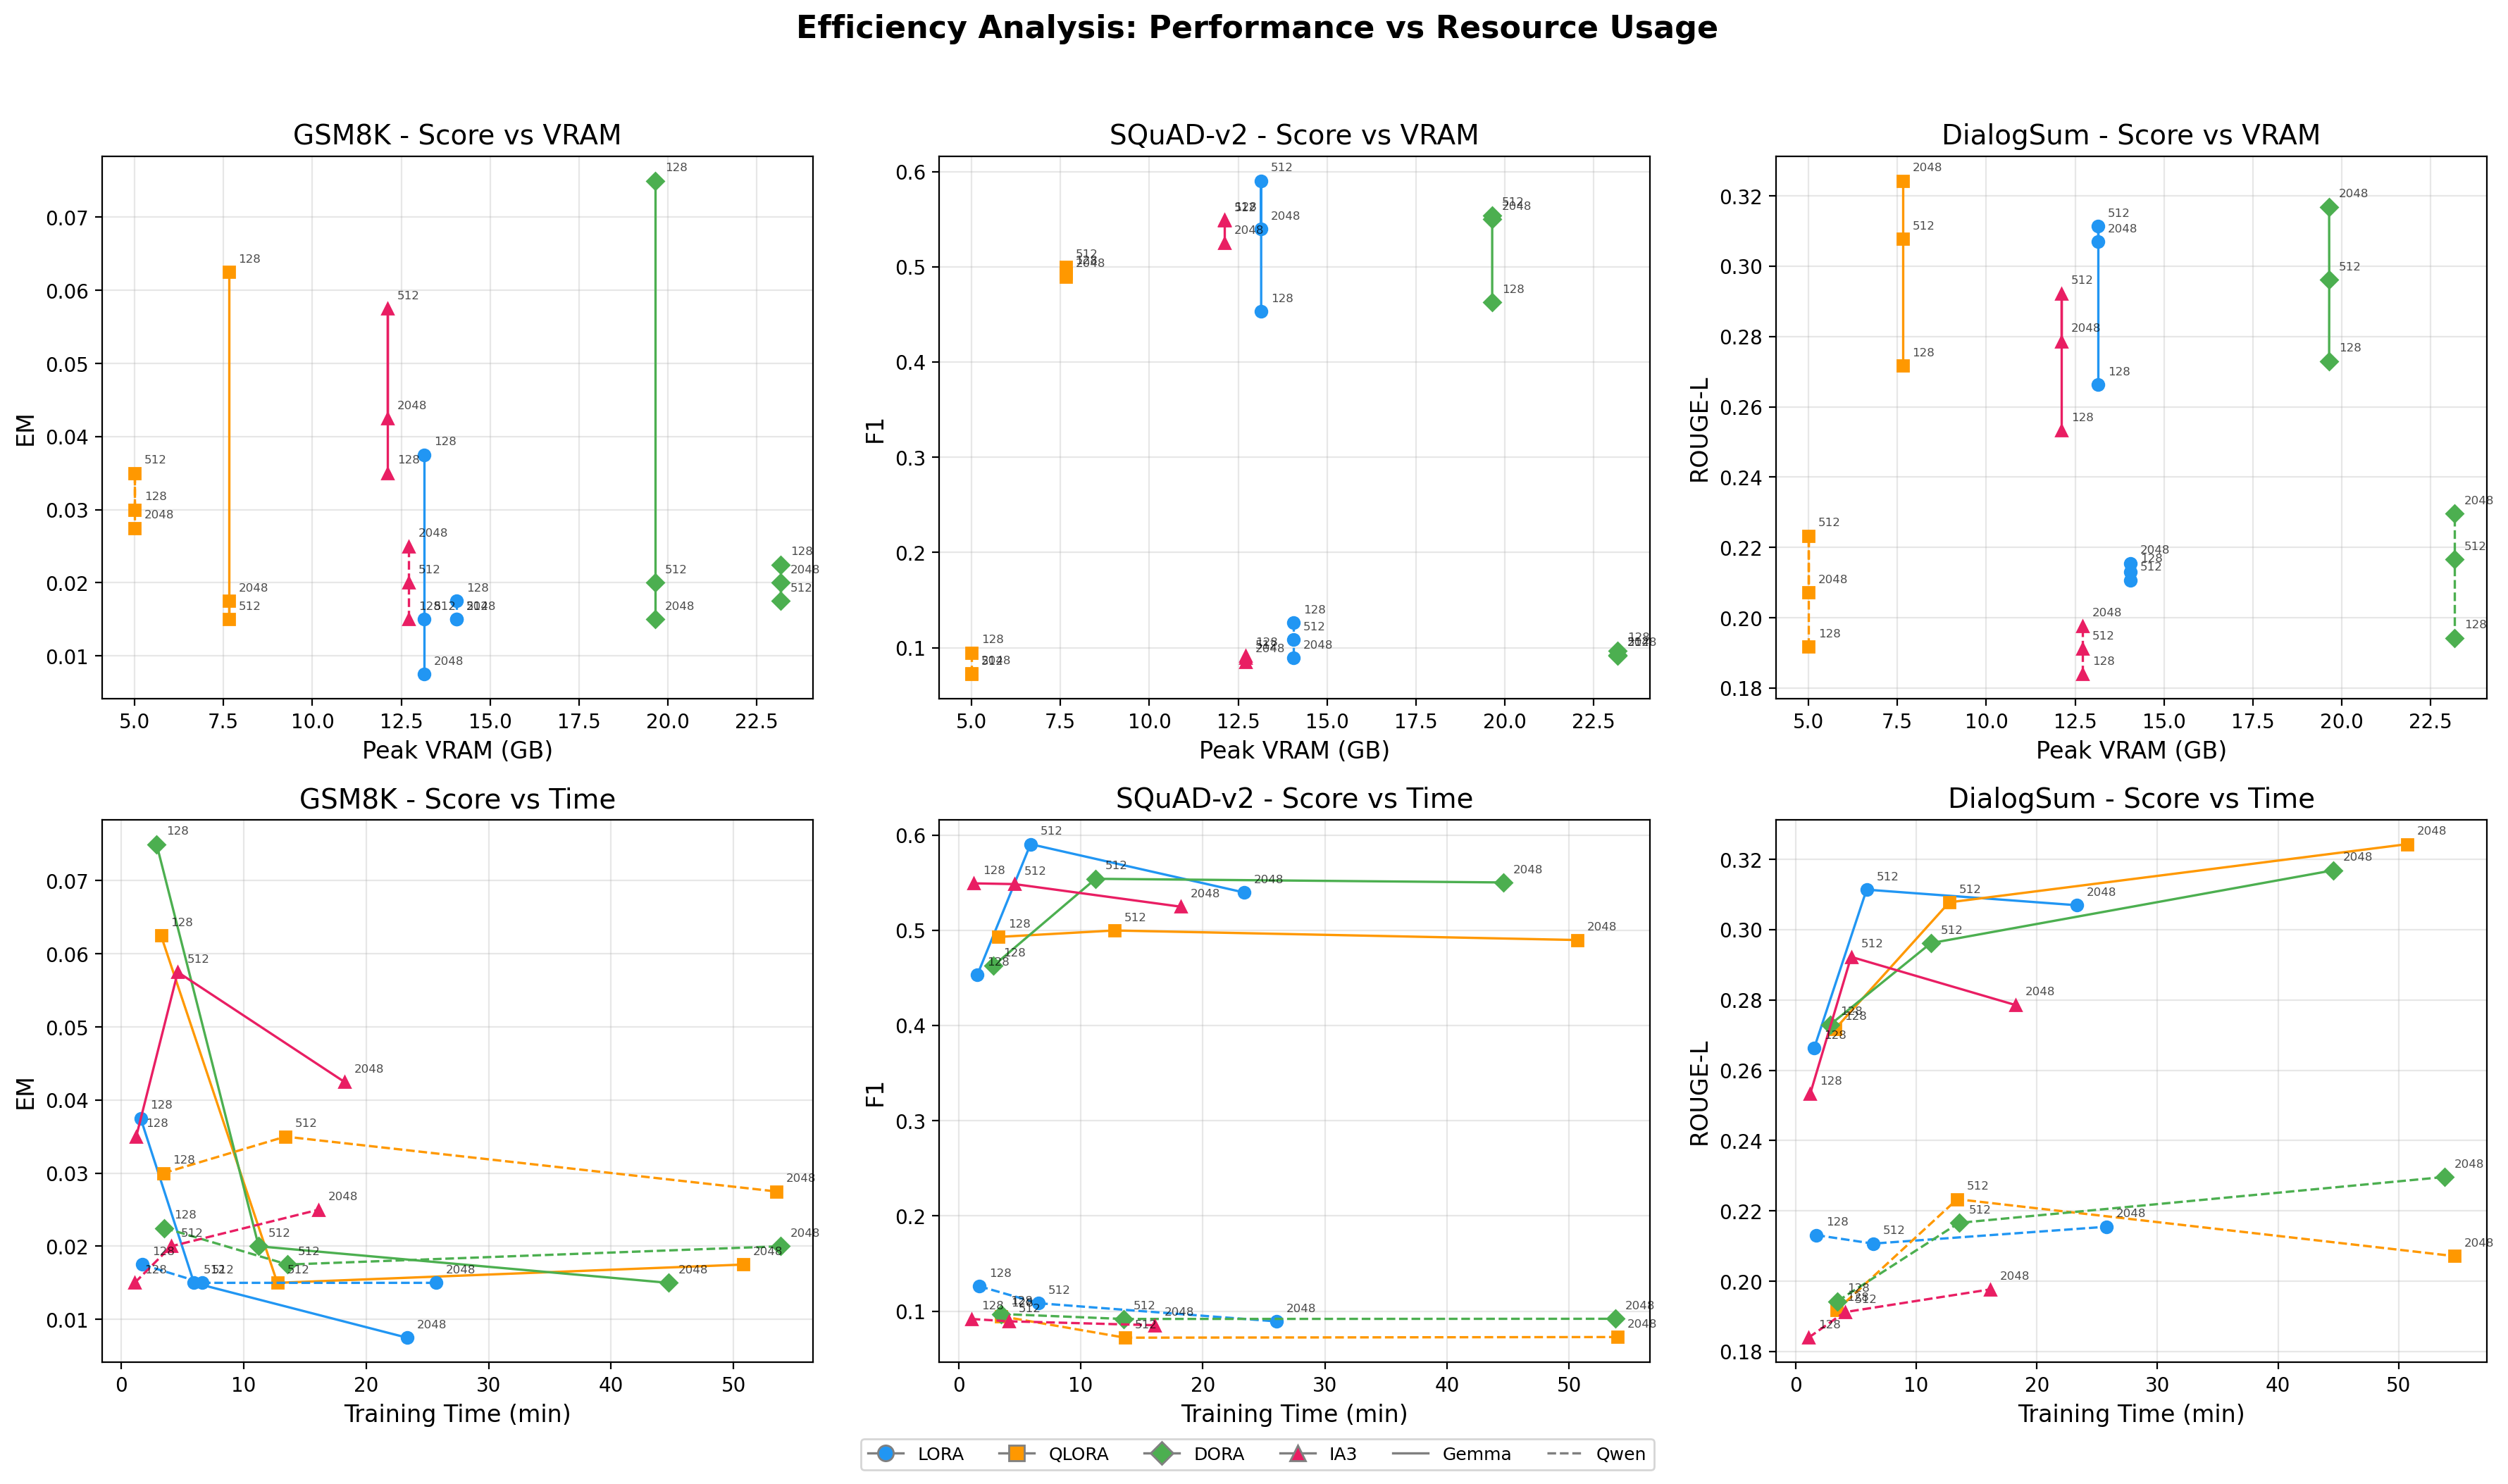
\includegraphics[width=0.7\textwidth]{figures/fig6_efficiency_scatter.png}
\caption{Efficiency analysis: task performance vs.\ resource consumption. Top row: score vs.\ peak VRAM. Bottom row: score vs.\ training time. Each point is annotated with its data budget (128, 512, or 2048). Solid lines represent Gemma, dashed lines represent Qwen. Points closer to the upper-left corner of each panel are more resource-efficient.}
\label{fig:efficiency}
\end{figure}

The Pareto analysis reveals several practical insights. On SQuAD-v2 (Gemma), the LoRA configuration at budget 512 achieves the best absolute score (F1 = 59.04\%) with moderate resource consumption (13.15 GB VRAM, $\sim$6 min), making it a strong practical choice. IA3 occupies the low-resource corner across all tasks, making it attractive when resources are extremely constrained, though at the cost of lower absolute performance. DoRA consistently appears in the high-resource region, justified only when it delivers the top score in a specific configuration (e.g., DialogSum on Qwen at budget 2048).

The budget annotations on each point reveal the scaling trajectory: increasing the budget moves points to the right (more time/VRAM) while also shifting them upward (higher score), but the slope of this trade-off varies by method. Methods with steeper slopes deliver more performance gain per unit of additional resource.

\subsubsection{Trainable Parameter Analysis}

The Pareto analysis highlights the trade-off between performance and resource consumption, but does not directly explain \emph{why} certain methods are more expensive than others. The answer lies in the trainable parameter count: methods with more parameters require larger optimizer states and more computation per gradient step. Figure~\ref{fig:params} visualizes the trainable parameter ratios that underlie the efficiency differences observed in Figures~\ref{fig:vram} and~\ref{fig:time}.

\begin{figure}[H]
\centering

\includegraphics[width=0.85\textwidth]{figures/fig7_trainable_params.png}
\caption{Trainable parameter ratios for each PEFT method. IA3 trains fewer than 0.02\% of total parameters, while QLoRA trains the highest proportion. The y-axis uses a logarithmic scale to accommodate the large range.}
\label{fig:params}
\end{figure}

The two-order-of-magnitude range in trainable parameters (from IA3's $\sim$0.01\% to QLoRA's $\sim$1.7\%) directly explains the efficiency patterns observed above. IA3's extreme parameter efficiency translates to both low VRAM (fewer optimizer states) and fast training (simpler gradient computation). Notably, QLoRA's higher trainable ratio does not translate to higher VRAM because the base model's 4-bit quantization more than compensates for the full-precision adapters. LoRA and DoRA have similar trainable ratios ($\sim$0.8--1.0\%), with DoRA being slightly higher due to the additional magnitude vector.

\subsection{Method Ranking Analysis}

To aggregate across all 18 configurations per model (3 tasks $\times$ 3 budgets $\times$ 2 seeds), we compute the average rank of each  PEFT method, where rank 1 indicates the best performer in a given configuration. This ranking-based view complements the per-task tables by summarizing method-level trends across the entire experiment matrix. A lower average rank indicates that a method wins more frequently; a rank of 2.5 would mean the method is equally likely to be first or third among the four methods.

Figure~\ref{fig:ranking} presents these rankings in three panels: overall (both models combined), Gemma-specific, and Qwen-specific. The overall panel provides the headline comparison, while the per-model panels reveal whether a method's strength is concentrated in one backbone or spread across both.
\begin{figure}[H]
\centering

\includegraphics[width=\textwidth]{figures/fig8_method_ranking.png}
\caption{Average method ranking across all configurations. Lower rank is better (rank 1 = best in that configuration). Left panel: overall ranking across both models. Middle and right panels: model-specific rankings. No method achieves a dominant rank below 2.0, confirming that method selection must be context-dependent.}
\label{fig:ranking}
\end{figure}

The ranking analysis confirms that no single method dominates. On Gemma, IA3 achieves the best average rank ($\sim$2.0), largely because it wins frequently at the smallest budget where its parameter efficiency is most valuable. On Qwen, the rankings are more evenly distributed, with no method clearly ahead. The overall ranking shows all four methods clustered between rank 2.0 and 3.0, reinforcing the central conclusion: PEFT selection must be based on the specific combination of task, budget, and model, not on a global leaderboard.

\subsection{Practical Guidelines}

Based on the full set of results, we summarize the following practical guidelines for PEFT method selection. These guidelines synthesize the performance, efficiency, and ranking findings discussed above into actionable recommendations.

\begin{itemize}
    \item \textbf{When GPU memory is the primary constraint, choose QLoRA first.} It is consistently the most memory-efficient method on both backbones, requiring as little as 5 GB for a 3B model.
    \item \textbf{When training speed is the primary concern, IA3 is the strongest default choice.} It achieves the fastest wall-clock training time (1--2 min at budget 128) and the smallest trainable parameter ratio (0.01\%).
    \item \textbf{For summarization tasks, method preference is strongly budget-dependent.} On both backbones, the best method changes as the training budget increases---practitioners should benchmark at their target budget rather than relying on results from a different budget.
    \item \textbf{For extractive QA, backbone choice matters more than PEFT choice.} Gemma substantially outperforms Qwen on SQuAD v2 across all budgets; the 4--5$\times$ F1 gap overwhelms the within-model method differences.
    \item \textbf{Do not rely on a single global method ranking.} The best PEFT method depends on the interaction among task type, supervision scale, and model family. Our 144-run matrix shows that the winning method changes across budget levels in 4 out of 6 model-task combinations.
    \item \textbf{For high-resource settings where performance is paramount, consider DoRA.} While it is the most resource-intensive method, DoRA wins in several high-budget configurations (e.g., DialogSum at budget 2048 on both models), suggesting that its magnitude-direction decomposition provides genuine expressiveness benefits when sufficient data is available.
\end{itemize}

Figure~\ref{fig:cost_summary} consolidates the resource cost picture for quick reference, combining VRAM and training time for all method-budget pairs on both models.

\begin{figure}[H]
\centering

\includegraphics[width=0.9\textwidth]{figures/fig10_cost_summary.png}
\caption{Training cost summary combining VRAM usage (top) and training time (bottom) for all method-budget combinations on both models. This figure can be used as a reference card when deciding which method-budget pair fits within a given resource constraint.}
\label{fig:cost_summary}
\end{figure}

\subsection{Limitations}

This study has several limitations. First, although we include two model families, the scope is still limited to medium-sized instruction-tuned LLMs; extrapolating to models exceeding 70B parameters may yield different patterns. Second, we evaluate only three task types, which cannot cover the full diversity of real-world adaptation scenarios such as code generation, multilingual translation, or tool-use. Third, the project focuses on PEFT comparison rather than comparison against full-parameter fine-tuning, so the conclusions are relative within the PEFT setting and do not address when PEFT is preferable to full fine-tuning. Fourth, our final report emphasizes aggregate matrix-level analysis rather than a complete step-level dynamics study for all 144 runs; a more detailed analysis of training dynamics (loss curves, early stopping behavior) could reveal additional insights. Fifth, evaluation is conducted on a fixed 200-example subset per task with short generation budgets and greedy decoding, which makes absolute scores (especially on GSM8K and SQuAD v2) sensitive to generation length, stop-token behavior, and lightweight answer-extraction rules; the reported numbers should therefore be read as comparative signals across methods rather than as definitive absolute benchmark scores. Finally, our learning rate tuning was performed on a single model-task-budget combination and transferred to all other settings; per-method hyperparameter optimization could change the relative rankings.

\section{Conclusion}

In this project, we conducted a controlled empirical study of four representative PEFT methods---LoRA, QLoRA, DoRA, and IA3---for instruction-tuned LLMs. By comparing two model families, three task types, and three data budgets in a 144-run experiment matrix, we showed that PEFT method preference is not universal. Instead, it depends on the interaction among supervision scale, task characteristics, and model architecture.

Our empirical results support three main conclusions. First, \textbf{no PEFT method dominates across all regimes}. The winning method changes with budget in 4 out of 6 model-task combinations, and no method achieves an average rank below 2.0 in our ranking analysis. Second, \textbf{efficiency differences are large and practically important}: QLoRA reduces peak VRAM by 3--5$\times$ compared to LoRA and DoRA, IA3 trains 2--4$\times$ faster than other methods, and DoRA requires the most resources in exchange for occasional performance gains. Third, \textbf{the most suitable method depends jointly on the target task, the available data budget, and the backbone model family}. These results suggest that PEFT selection should be framed as a conditional decision problem rather than a single leaderboard comparison.

Additional base-model evaluation further shows that PEFT does not deliver uniform gains across all tasks. The improvements are most substantial on summarization (ROUGE-L +0.074) and reasoning (EM +0.065), where even limited fine-tuning can meaningfully shift generation behavior. On SQuAD v2, the backbone model itself explains a large share of the final performance, suggesting that practitioners should first verify whether fine-tuning is warranted relative to the no-adaptation baseline.

The main practical challenges in this project were experiment management under HPC queue limits, method-specific resource differences, and ensuring consistent evaluation across a large experiment matrix. Future work can extend this framework to larger model scales (e.g., 13B and 70B), more diverse instruction tasks (code generation, multilingual settings), a more systematic training-dynamics analysis with learning curve visualization, and the inclusion of full fine-tuning baselines to contextualize the PEFT results.

\section{Contributions}

% Default split: even 25\% each across the four team members listed on the title page.
% Update names-to-roles and percentages before final submission if the actual split differs.
The estimated contribution of each team member is as follows:
\begin{itemize}
    \item Meijun Liu: 25\% --- project design, training framework, experiment management.
    \item Xiaoqian Jiao: 25\% --- data preparation, preprocessing, budget construction.
    \item Yiying Pan: 25\% --- evaluation scripts, result aggregation, plotting.
    \item Rui Liu: 25\% --- writing, report integration, presentation preparation.
\end{itemize}

The total contribution sums to 100\%.

\bibliographystyle{plain}
\bibliography{references}

\appendix

\section{Supplementary Result Tables}

This appendix includes supplementary result tables that are not shown in the main text. We report mean $\pm$ standard deviation over two seeds for the main task metrics. Additionally, all source code and raw experimental results of this work are publicly available at: \href{https://github.com/aliciamj613/dsaa-peft-handoff}{https://github.com/aliciamj613/dsaa-peft-handoff}.


\begin{table}[H]
\centering
\small
\caption{GSM8K EM (mean $\pm$ std over two seeds).}
\begin{tabular}{llccc}
\toprule
Model & Method & 128 & 512 & 2048 \\
\midrule
\multirow{4}{*}{Gemma-2-2B-it} & LoRA & 0.0375 $\pm$ 0.0035 & 0.0150 $\pm$ 0.0000 & 0.0075 $\pm$ 0.0035 \\
 & QLoRA & 0.0625 $\pm$ 0.0106 & 0.0150 $\pm$ 0.0000 & 0.0175 $\pm$ 0.0106 \\
 & DoRA & 0.0750 $\pm$ 0.0141 & 0.0200 $\pm$ 0.0071 & 0.0150 $\pm$ 0.0000 \\
 & IA3 & 0.0350 $\pm$ 0.0000 & 0.0575 $\pm$ 0.0035 & 0.0425 $\pm$ 0.0035 \\
\midrule
\multirow{4}{*}{Qwen2.5-3B-Instruct} & LoRA & 0.0175 $\pm$ 0.0035 & 0.0150 $\pm$ 0.0071 & 0.0150 $\pm$ 0.0141 \\
 & QLoRA & 0.0300 $\pm$ 0.0141 & 0.0350 $\pm$ 0.0141 & 0.0275 $\pm$ 0.0106 \\
 & DoRA & 0.0225 $\pm$ 0.0035 & 0.0175 $\pm$ 0.0035 & 0.0200 $\pm$ 0.0000 \\
 & IA3 & 0.0150 $\pm$ 0.0071 & 0.0200 $\pm$ 0.0071 & 0.0250 $\pm$ 0.0071 \\
\bottomrule
\end{tabular}
\end{table}

\begin{table}[H]
\centering
\small
\caption{DialogSum ROUGE-L (mean $\pm$ std over two seeds).}
\begin{tabular}{llccc}
\toprule
Model & Method & 128 & 512 & 2048 \\
\midrule
\multirow{4}{*}{Gemma-2-2B-it} & LoRA & 0.2662 $\pm$ 0.0021 & 0.3114 $\pm$ 0.0018 & 0.3069 $\pm$ 0.0066 \\
 & QLoRA & 0.2717 $\pm$ 0.0021 & 0.3078 $\pm$ 0.0039 & 0.3243 $\pm$ 0.0104 \\
 & DoRA & 0.2730 $\pm$ 0.0074 & 0.2961 $\pm$ 0.0026 & 0.3169 $\pm$ 0.0192 \\
 & IA3 & 0.2533 $\pm$ 0.0018 & 0.2922 $\pm$ 0.0004 & 0.2786 $\pm$ 0.0014 \\
\midrule
\multirow{4}{*}{Qwen2.5-3B-Instruct} & LoRA & 0.2131 $\pm$ 0.0001 & 0.2107 $\pm$ 0.0039 & 0.2155 $\pm$ 0.0011 \\
 & QLoRA & 0.1917 $\pm$ 0.0002 & 0.2233 $\pm$ 0.0011 & 0.2071 $\pm$ 0.0027 \\
 & DoRA & 0.1943 $\pm$ 0.0015 & 0.2166 $\pm$ 0.0037 & 0.2297 $\pm$ 0.0017 \\
 & IA3 & 0.1839 $\pm$ 0.0012 & 0.1912 $\pm$ 0.0005 & 0.1977 $\pm$ 0.0014 \\
\bottomrule
\end{tabular}
\end{table}

\begin{table}[H]
\centering
\small
\caption{SQuAD v2 F1 (mean $\pm$ std over two seeds).}
\begin{tabular}{llccc}
\toprule
Model & Method & 128 & 512 & 2048 \\
\midrule
\multirow{4}{*}{Gemma-2-2B-it} & LoRA & 0.4529 $\pm$ 0.0308 & 0.5904 $\pm$ 0.0286 & 0.5397 $\pm$ 0.0204 \\
 & QLoRA & 0.4929 $\pm$ 0.0150 & 0.4997 $\pm$ 0.0102 & 0.4897 $\pm$ 0.0249 \\
 & DoRA & 0.4629 $\pm$ 0.0048 & 0.5540 $\pm$ 0.0299 & 0.5502 $\pm$ 0.0177 \\
 & IA3 & 0.5493 $\pm$ 0.0035 & 0.5484 $\pm$ 0.0000 & 0.5247 $\pm$ 0.0012 \\
\midrule
\multirow{4}{*}{Qwen2.5-3B-Instruct} & LoRA & 0.1262 $\pm$ 0.0088 & 0.1084 $\pm$ 0.0013 & 0.0893 $\pm$ 0.0020 \\
 & QLoRA & 0.0947 $\pm$ 0.0003 & 0.0722 $\pm$ 0.0167 & 0.0729 $\pm$ 0.0110 \\
 & DoRA & 0.0971 $\pm$ 0.0013 & 0.0918 $\pm$ 0.0136 & 0.0920 $\pm$ 0.0031 \\
 & IA3 & 0.0918 $\pm$ 0.0010 & 0.0894 $\pm$ 0.0001 & 0.0853 $\pm$ 0.0008 \\
\bottomrule
\end{tabular}
\end{table}





\end{document}
